\documentclass[../manuale-utente.tex]{subfiles}

\begin{document}

\subsection{Requisiti}%
\label{sub:requisiti}

\begin{description}
    \item[Browser:] Google Chrome 50, Firefox 48, Safari 9.1.
    \item[Necessario:] JavaScript.
\end{description}


\subsection{Manuale d'uso}%
\label{sub:manuale-uso-web}

\subsubsection{Pagina home}%
\label{subs:pagina-home}

\begin{figure}[H]
    \centering
    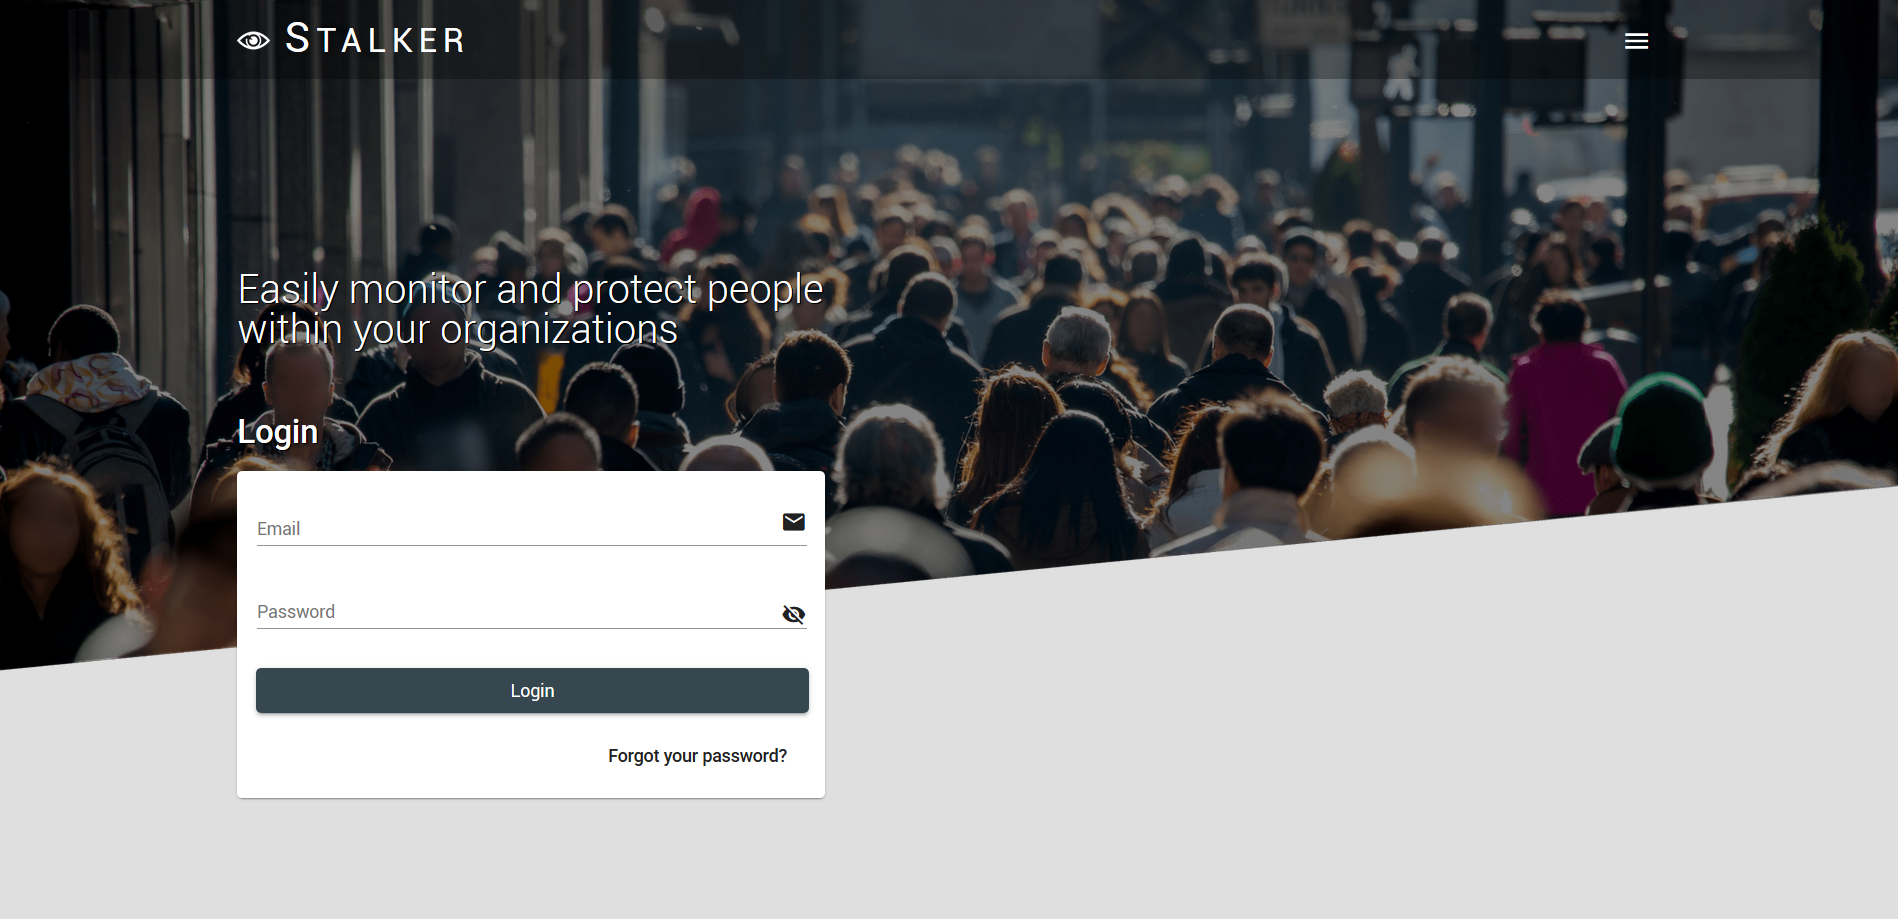
\includegraphics[width=175mm]{img/web-app/pagina-home.PNG}
    \caption{Pagina di accesso}%
    \label{fig:web-app-pagina-accesso}
\end{figure}

La prima volta che viene aperta la web application di Stalker, l'utente viene indirizzato alla pagina principale (Home) che si trova al link \textit{localhost:4200/home}.

L'utente non è autenticato e ha tre possibilità:
\begin{itemize}
    \item essere registrato alla web app di Stalker e accedere con le proprie credenziali email e password (~\ref{fig:web-app-accesso} ).
    \item recuperare la password nel caso l'abbia smarrita (~\ref{fig:web-app-recupero-password} ).
    \item selezionare il menu ad hamburger posizionato sulla barra superiore a destra, per visualizzare le informazioni riguardo a Stalker.
\end{itemize} 
\newpage

\paragraph{Accesso alla web application}%
\label{par:accesso-alla-web-application}

\begin{figure}[H]
    \centering
    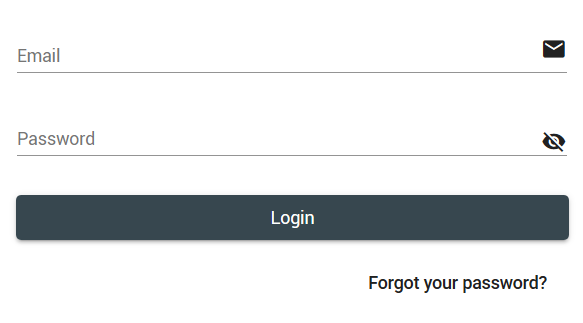
\includegraphics[width=120mm]{img/web-app/accesso-web-app.png}
    \caption{Pagina di registrazione}%
    \label{fig:web-app-accesso}
\end{figure}

L'utente vuole accedere al sistema di Stalker, quindi deve eseguire tre passaggi:
\begin{itemize}
    \item inserire correttamente l'email.
    \item inserire la password, e possibilmente visualizzarla durante la sua digitazione cliccando sulla figura a fine riga, che deve contenere almeno 8 caratteri alfanumerici e al massimo ne può contenere 32.
    \item selezionare il pulsante \textbf{Login} per inviare le credenziali al server.
\end{itemize} 

% E' corretto?
Nel caso l'operazione venga svolta correttamente, si avrà diritto all'accesso nella web application di Stalker, visualizzando la pagina del profilo personale (~\ref{fig:web-app-visualizza-profilo-personale} ).

In caso contrario, l'utente non è autorizzato, in quanto la procedura è fallita.

Le cause possono essere le seguenti:
\begin{itemize}
    \item l'email inserita non rispetta i vincoli imposti dal sistema di Stalker.
    \item la password non rispetta i vincoli imposti dal sistema di Stalker.
    \item l'email e la password inserite non rispettano i vincoli imposti dal sistema di Stalker.
    \item l'email inserita rispetta i vincoli, ma non è presente all'interno del database di Stalker.
    \item la password inserita rispetta i vincoli, ma non è presente all'interno del database di Stalker.
    \item l'email e la password inserite rispettano i vincoli, ma non sono presenti all'interno del database di Stalker.
\end{itemize}

In ogni caso, il messaggio di errore non sarà specifico ma generico, per motivi di sicurezza.
\newpage

\paragraph{Recupero password}%
\label{par:recupero-password}

\begin{figure}[H]
    \centering
    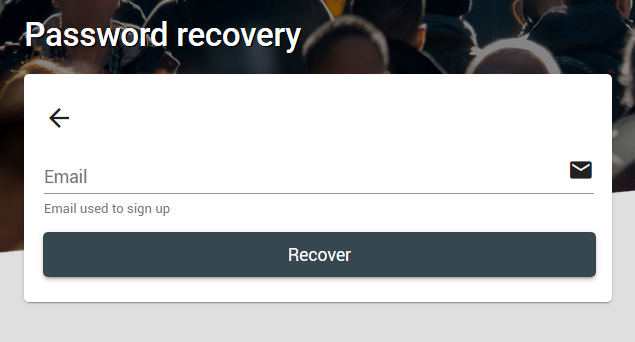
\includegraphics[width=150mm]{img/web-app/recupero-password.PNG}
    \caption{Recupero password}%
    \label{fig:web-app-recupero-password}
\end{figure}

L'utente ha smarrito la password o non se la ricorda più, quindi deve eseguire tre passaggi:
\begin{itemize}
    \item cliccare alla voce \textbf{Forgot your password?} presente nel form per l'accesso alla web application (~\ref{fig:web-app-pagina-accesso} ).
    \item inserire correttamente l'email.
    \item selezionare il pulsante \textbf{Recover} per inviare la richiesta al server.
\end{itemize}

Nel caso l'operazione venga svolta correttamente, l'utente riceverà una mail sulla propria casella postale contenente il link per il recupero della password.

In caso contrario, l'utente non può recuperare la password, in quanto la procedura è fallita.

Le cause possono essere le seguenti:
\begin{itemize}
    \item l'email inserita non rispetta i vincoli imposti dal sistema di Stalker.
    \item l'email inserita rispetta i vincoli, ma non è presente nel database di Stalker, quindi non si può avviare la procedura.
\end{itemize}

In ogni caso, il messaggio di errore non sarà specifico ma generico, per motivi di sicurezza.
\newpage

\subsubsection{Visualizza profilo personale}%
\label{subs:visualizza-profilo-personale}

\begin{figure}[H]
    \centering
    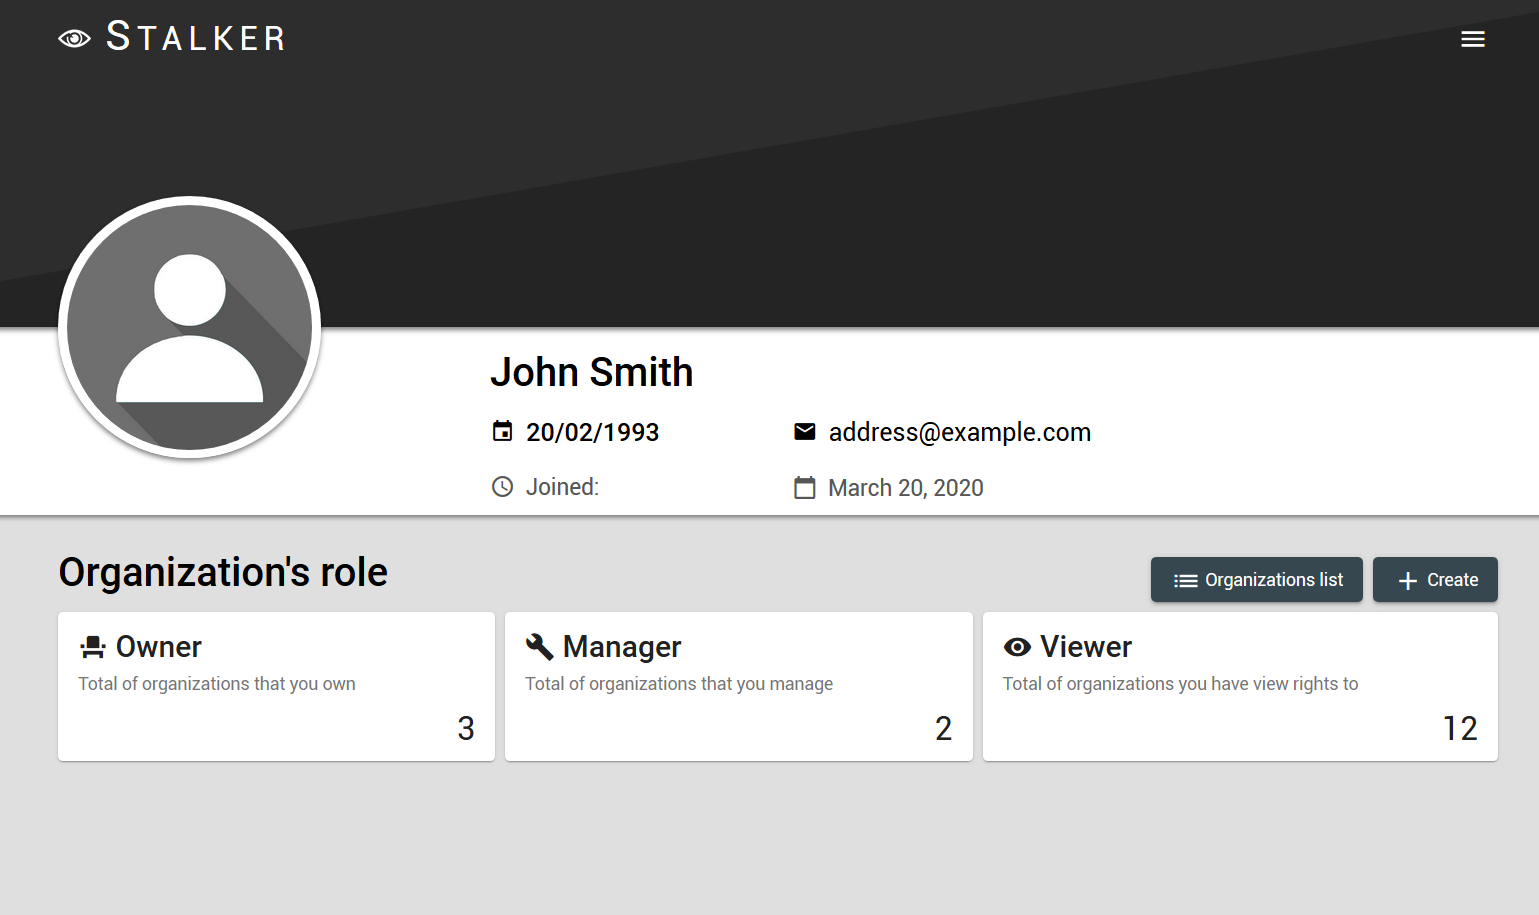
\includegraphics[width=120mm]{img/web-app/visualizza-profilo-personale.PNG}
    \caption{Visualizza profilo personale}%
    \label{fig:web-app-visualizza-profilo-personale}
\end{figure}

\textbf{Endpoint}: localhost:4200/users/:id
Lorem ipsum
\newpage

\subsubsection{Visualizza organizzazioni}%
\label{subs:visualizza-organizzazioni}

% \begin{figure}[H]
%     \centering
%     \includegraphics[width=120mm]{img/web-app/visualizza-organizzazioni.png}
%     \caption{Visualizza organizzazioni}%
%     \label{fig:web-app-visualizza-organizzazioni}
% \end{figure}

\textbf{Endpoint}: localhost:4200/organizations
Lorem ipsum
\newpage

\paragraph{Visualizza dettagli organizzazione}%
\label{par:visualizza-dettagli-organizzazione}

\begin{figure}[H]
    \centering
    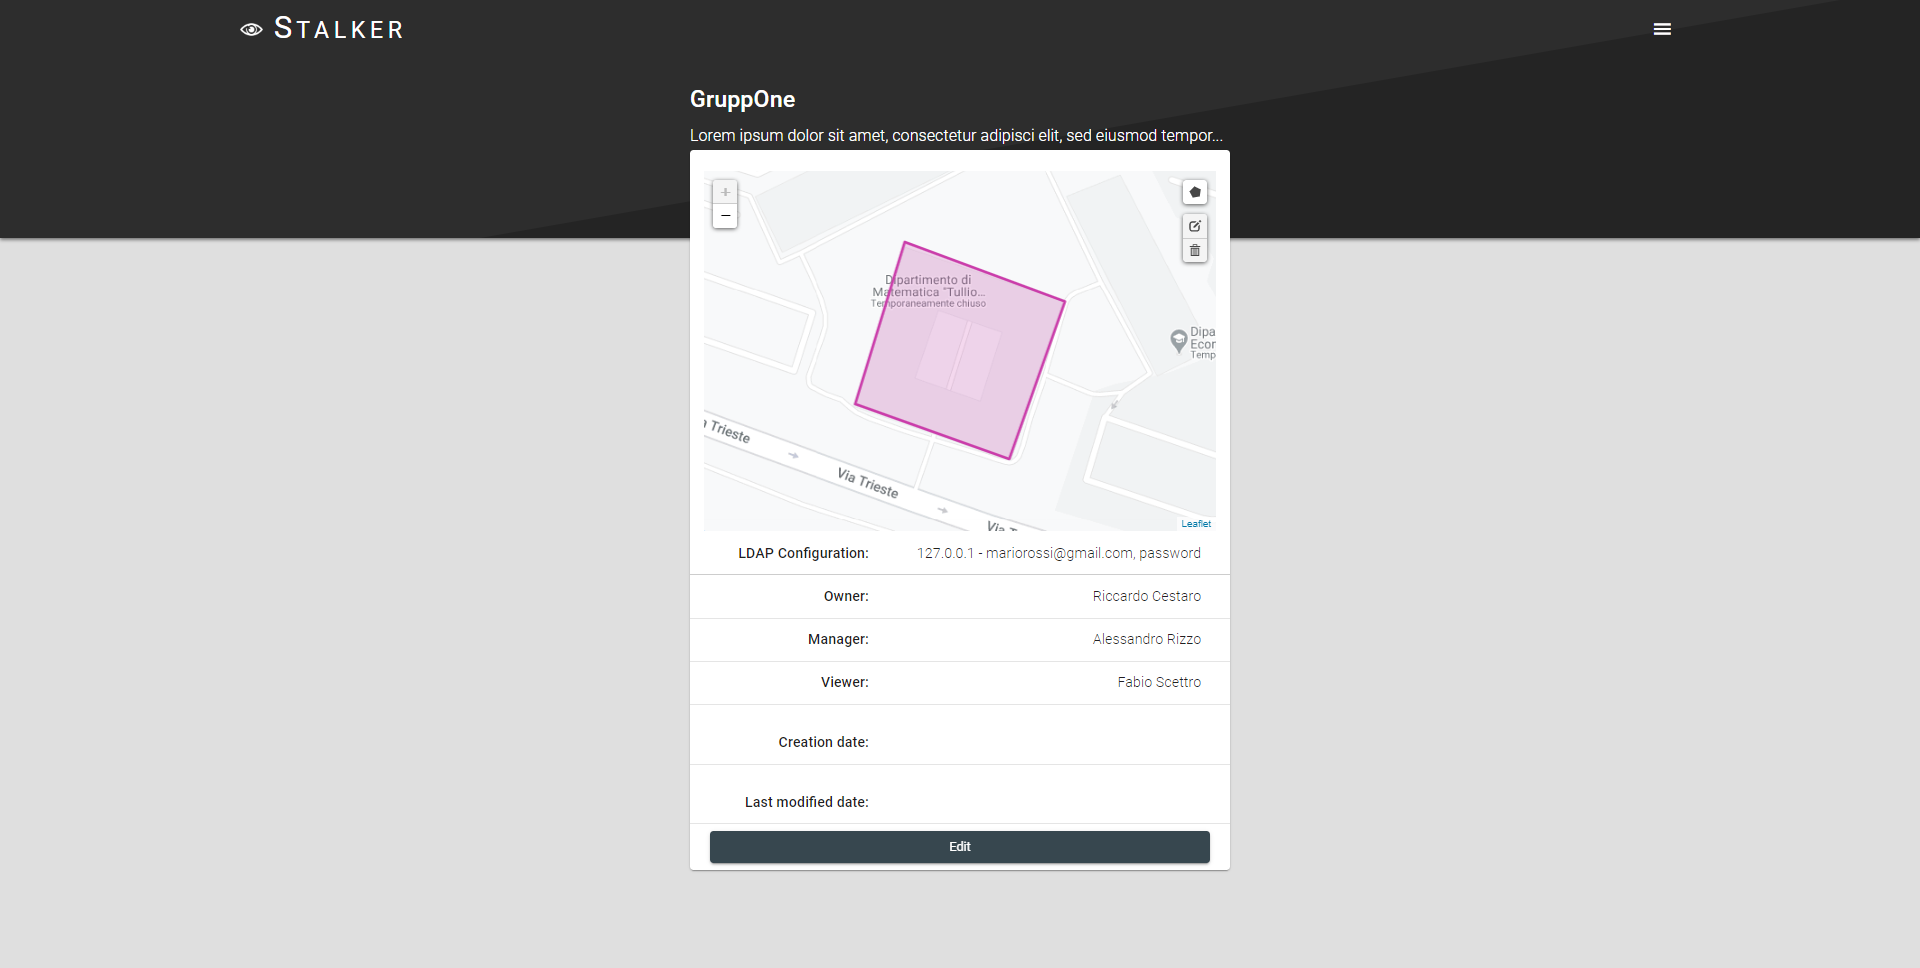
\includegraphics[width=120mm]{img/web-app/visualizza-dettagli-organizzazione.png}
    \caption{Visualizza dettagli organizzazione}%
    \label{fig:web-app-visualizza-dettagli-organizzazione}
\end{figure}

\textbf{Endpoint}: localhost:4200/organizations/:id
Lorem ipsum
\newpage

% Visualizza: (aggiungere un'immagine per ogni funzionalità) --> edit-organization
% - luoghi da una mappa interattiva
% - LDAP configuration
% - managers, owners e viewers
% - ecc..


\subsubsection{Modifica dettagli organizzazione}%
\label{subs:modififica-dettagli-organizzazione}

% \begin{figure}[H]
%     \centering
%     \includegraphics[width=120mm]{img/web-app/modifica-dettagli-organizzazione.png}
%     \caption{Modifica dettagli organizzazione}%
%     \label{fig:web-app-modifica-dettagli-organizzazione}
% \end{figure}

\textbf{Endpoint}: localhost:4200/organizations/:id/edit
Lorem ipsum
\newpage

% add other functionalities 

\end{document}
